\section{Paths and Connectivity}
Graphs are similar to train networks or airline routes. They connect one 
location to another.

\begin{Def}[Graph]

    A \textbf{graph} is a collection of points, called \textbf{vertices} or \textbf{nodes}, 
    connected by lines, called \textbf{edges}. Similarly to how a polygon has vertices connected by edges.

\end{Def}
\begin{Def}[Undirected Graph]

    An \textbf{undirected graph} is a graph where the edges have no particular direction going both ways between nodes. 
    A \textbf{degree} of a node is the number of edges connected to it.
\end{Def}
\noindent
\textbf{Example:} Figure (\ref{fig:undir_graph}) shows an undirected graph:\\
\begin{figure}[h]
    \begin{center}
      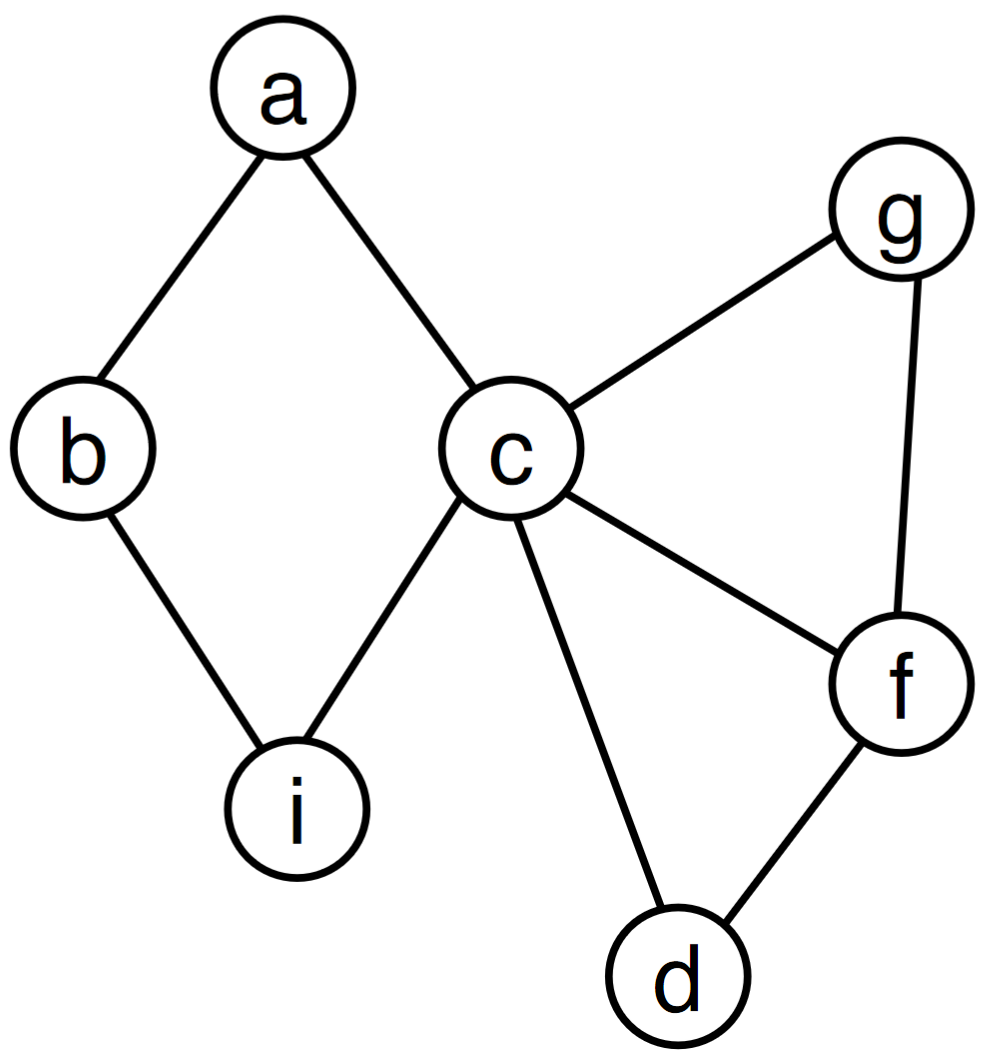
\includegraphics[height=1.8in]{./Sections/graphs/undir_graph.png}
    \end{center}
     \caption{An undirected graph with 7 vertices and 9 edges.}\label{fig:undir_graph}
  \end{figure}

\noindent
Node $a$ has a degree of 3, and node $c$ has a degree of 4.\\
\newpage

\begin{Def}[Directed Graph]

    A \textbf{directed graph} is where the edges have a specific direction from one node to another.
    \begin{itemize}
        \item  The \textbf{indegree} of a node is the number of edges that point to it.
        \item The \textbf{outdegree} of a node is the number of edges that point from it.
    \end{itemize}
\end{Def}
\noindent
\textbf{Example:} Figure (\ref{fig:dir_graph}) shows a directed graph:\\
\begin{figure}[h]
    \begin{center}
      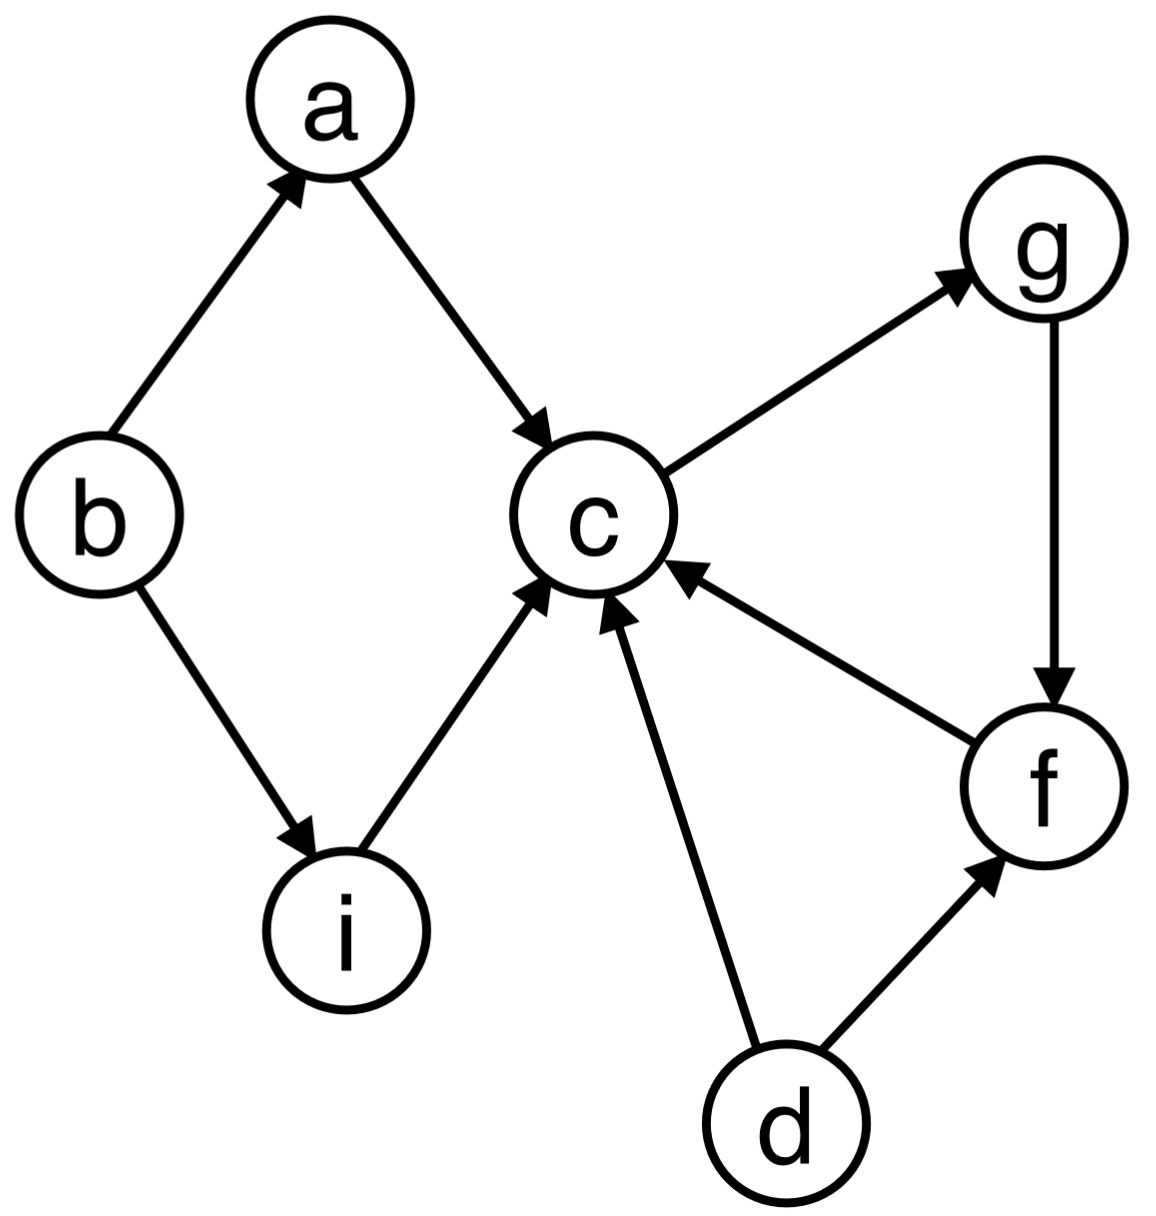
\includegraphics[height=1.5in]{./Sections/graphs/dir_graph.png}
    \end{center}
     \caption{A directed graph with 7 vertices and 9 edges.}\label{fig:dir_graph}
  \end{figure}

  \noindent
    Node $b$ has an outdegree of 2 and an indegree of 0. $c$ has an indegree of 4 and an outdegree of 1.

\begin{Def}[Weighted Graph]

    A \textbf{weighted graph} is a graph where each edge has a numerical value assigned to it.
\end{Def}
\noindent
\textbf{Example:} Figure (\ref{fig:weight_graph}) shows a weighted graph:\\
\begin{figure}[h]
    \begin{center}
      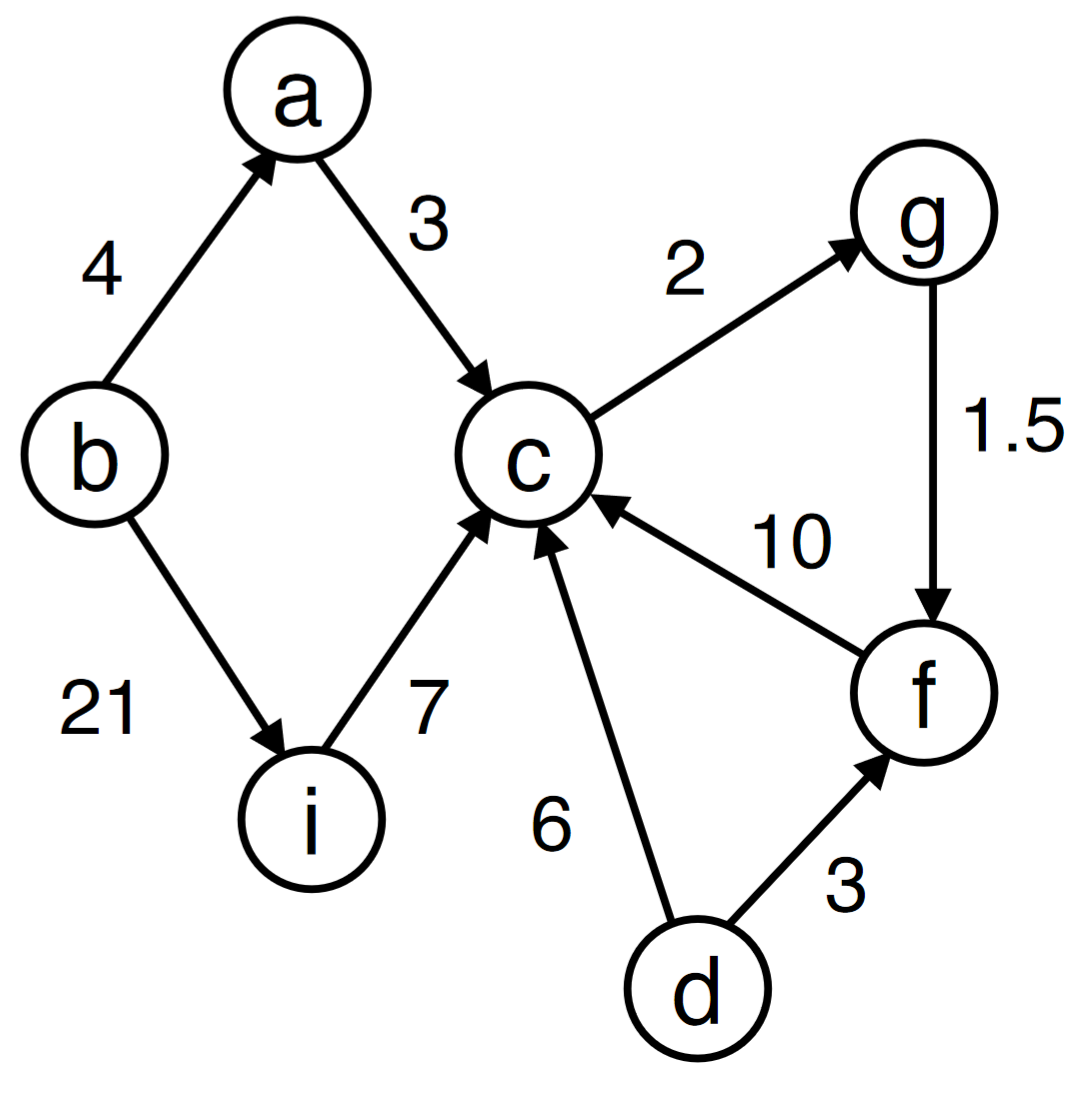
\includegraphics[height=1.5in]{./Sections/graphs/weight_graph.png}
    \end{center}
     \caption{A weighted graph with 7 vertices and 9 edges.}\label{fig:weight_graph}
  \end{figure}
\newpage
\begin{Def}[Path]

    A \textbf{path} is a sequence of edges that connect a sequence of vertices. A 
    path is \textbf{simple} if all nodes are distinct.
\end{Def}

\noindent
\textbf{Example:} In Figure (\ref{fig:path_graph}), a simple path $h\leftrightarrow b \leftrightarrow i \leftrightarrow c \leftrightarrow d$ is shown:\\
\begin{figure}[h]
    \begin{center}
      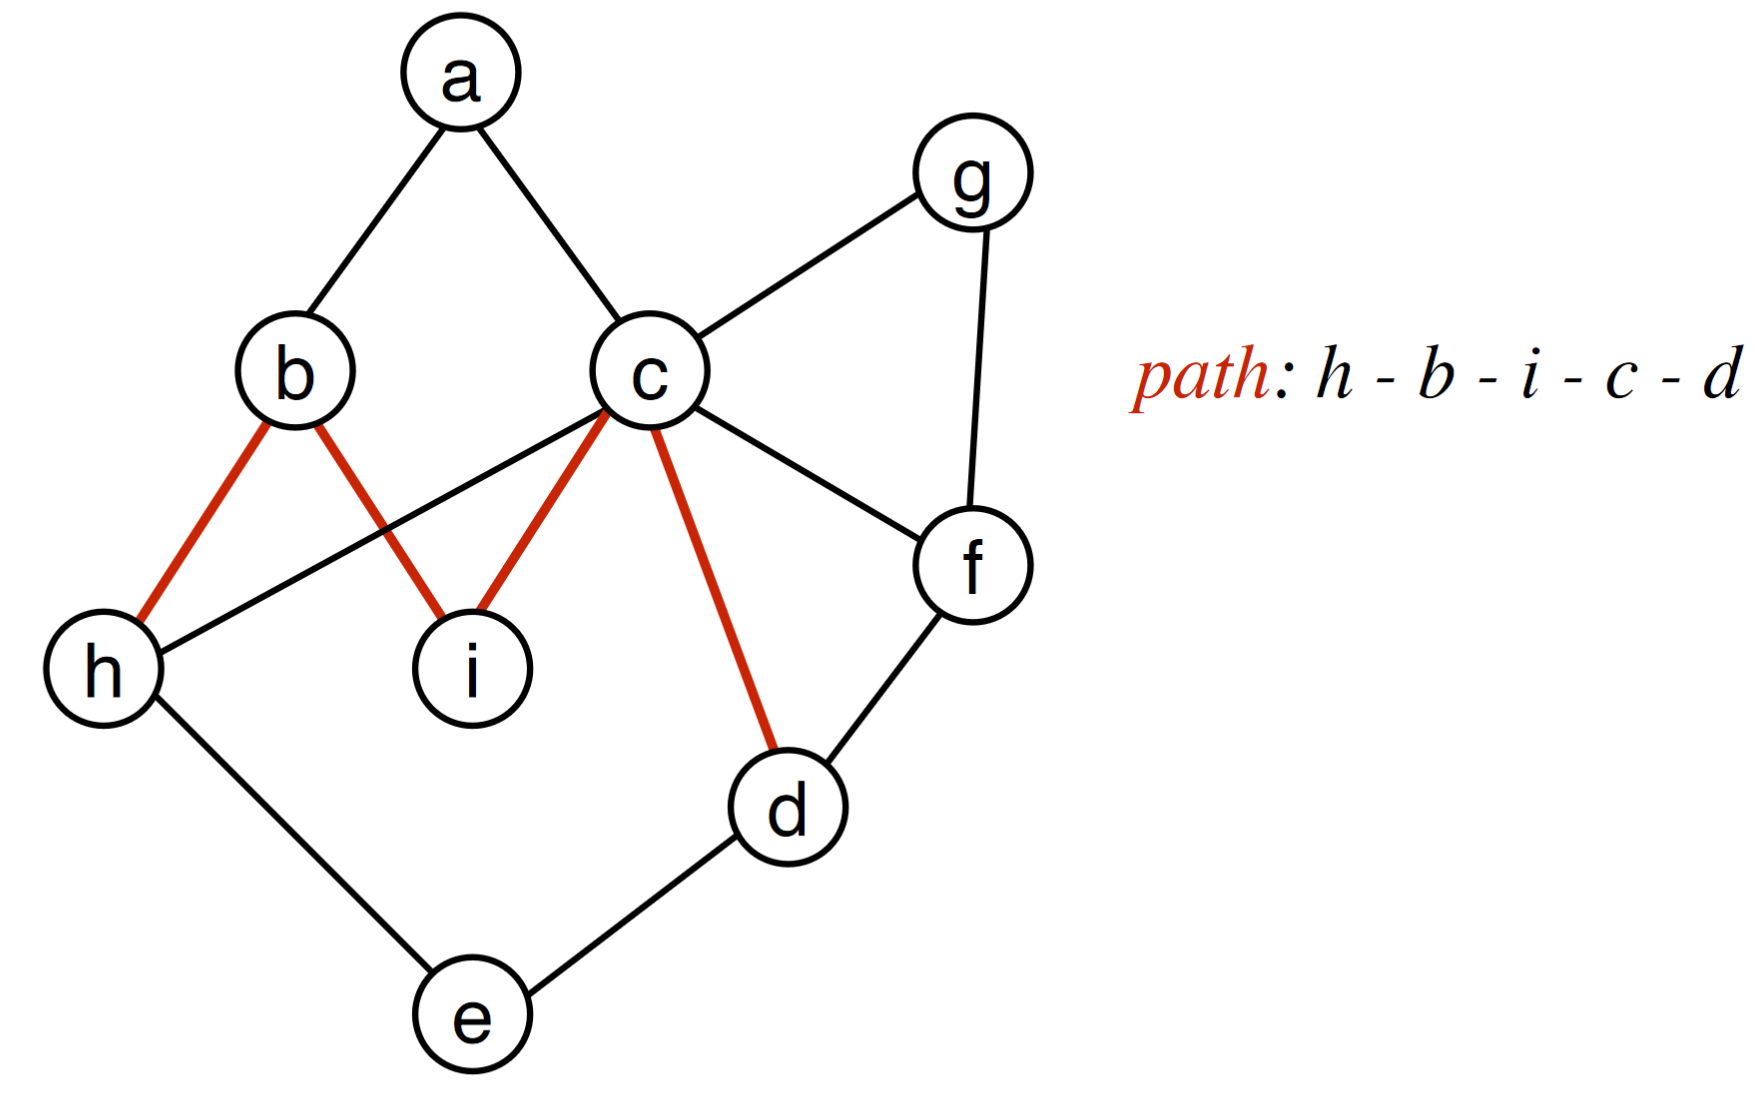
\includegraphics[height=1.8in]{./Sections/graphs/path_graph.png}
    \end{center}
     \caption{A graph with a simple path from $h$ to $d$.}\label{fig:path_graph}
  \end{figure}

\begin{Def}[Connectivity]

    A graph is \textbf{connected} if there is a path between every pair of vertices.\\
    A graph is \textbf{disconnected} if there are two vertices with no path between them.\\
    \underline{Connected graphs of $n$ nodes have at least $n-1$ edges.}
\end{Def}
\begin{figure}[h]
    \begin{center}
      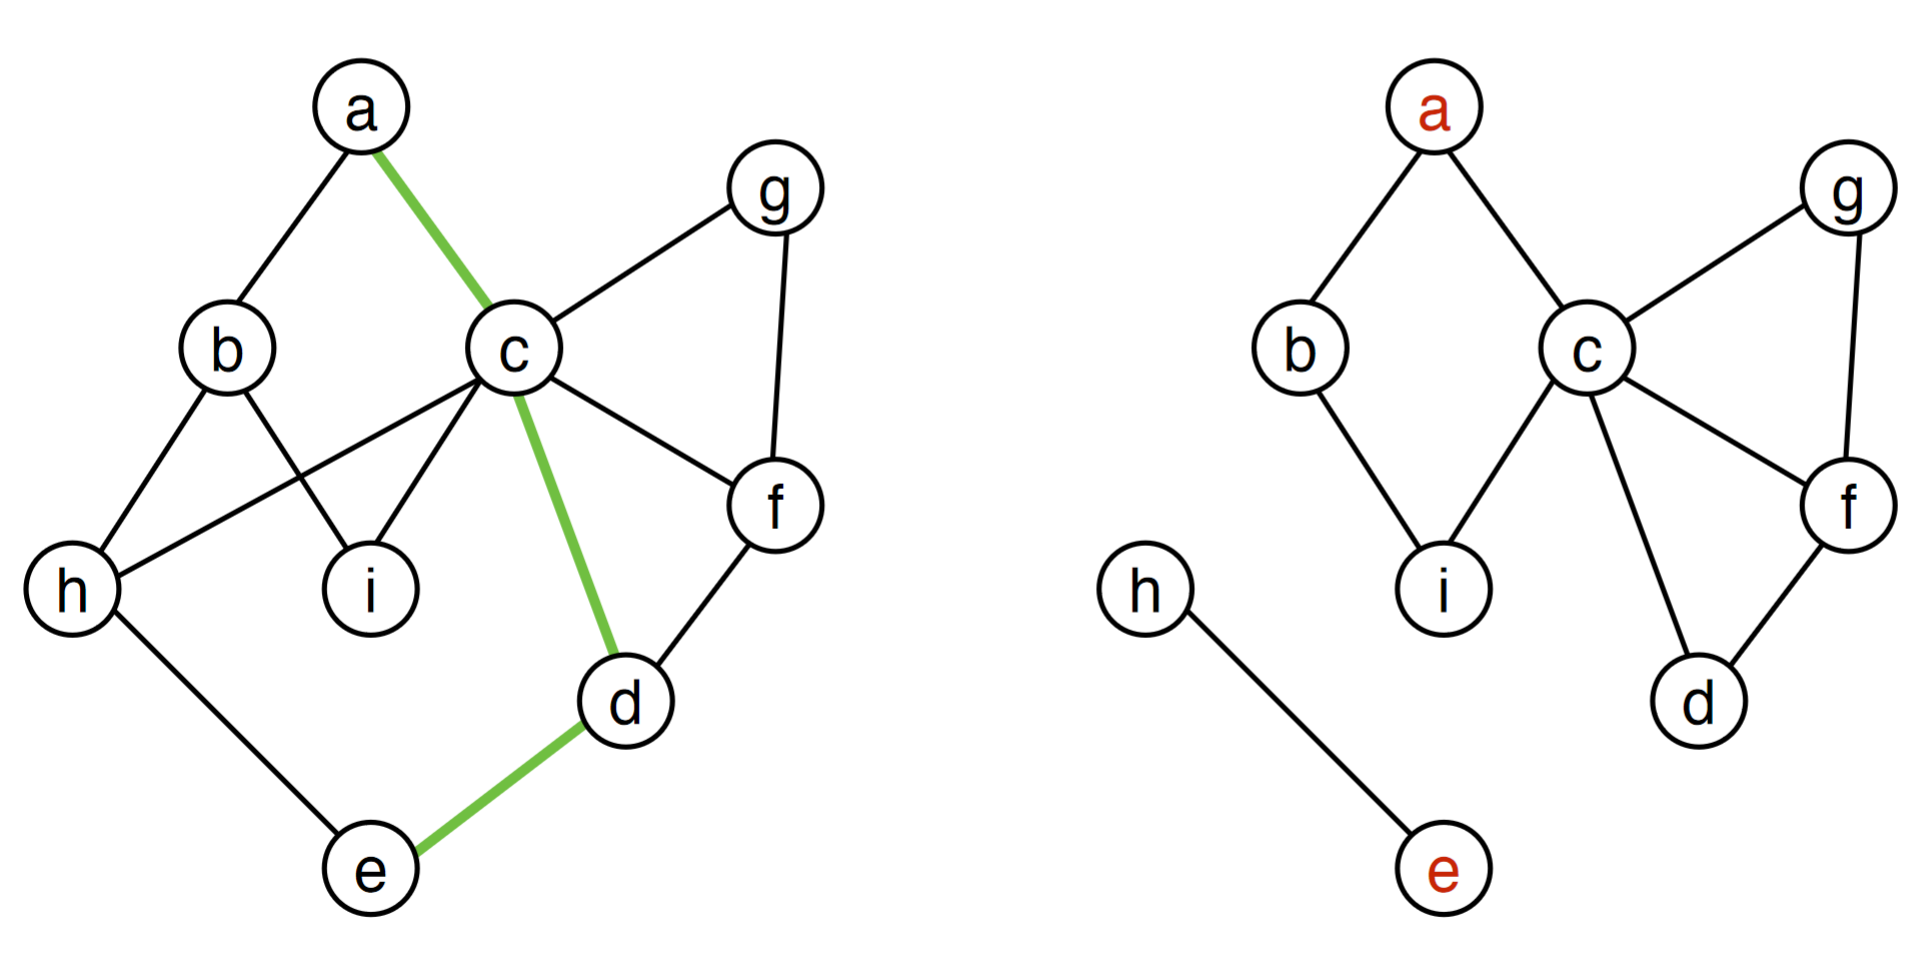
\includegraphics[height=1.8in]{./Sections/graphs/con_graph.png}
    \end{center}
     \caption{A connected graph $a\leftrightarrow c \leftrightarrow d \leftrightarrow e$  and disconnected graph.}\label{fig:con_graph}
  \end{figure}

  \newpage
  \begin{Def}[Adjacency Matrix]
      
      An \textbf{adjacency matrix} is an $n\times n$ matrix where such that $A[i][j] = 1$ if there is an edge between nodes $i$ and $j$.

  \end{Def}

  
\begin{figure}[h]
  \begin{center}
    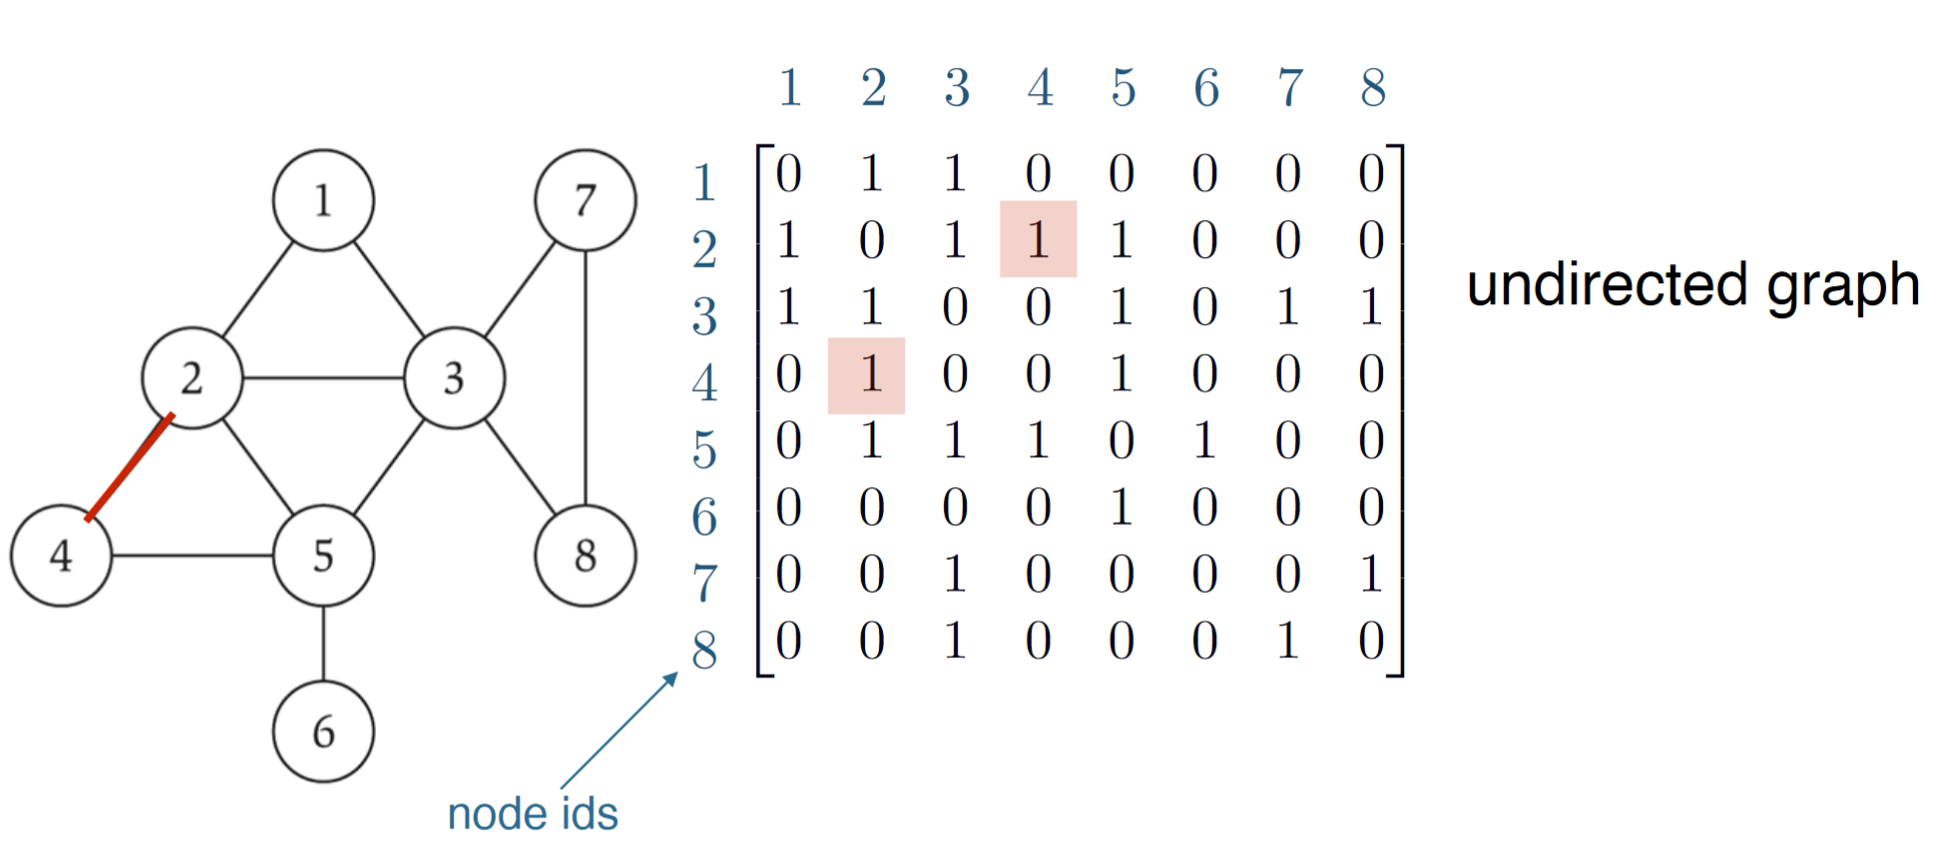
\includegraphics[height=1.5in]{./Sections/graphs/adj_matrix.png}
  \end{center}
   \caption{An adjacency matrix where the path $4\leftrightarrow2$ is highlighted ($A[2][4]$ or $A[4][2]$)}\label{fig:adj_matrix}
\end{figure}
\begin{theo}[Properties of Adjacency Matrix]

  The following properties hold for adjacency matrices:
    \begin{itemize}
        \item An undirected graph is symmetric about the diagonal.
        \item A directed graph is not symmetric about.
        \item A weighted graph has the weight of the edge instead of binary.
    \end{itemize}
    \noindent
    \textbf{Space Complexity:} $\Theta (n^2)$; \textbf{Time Complexities:}\\
    \textbf{Index edge $A[i][j]$:} $\Theta (1)$; \textbf{List neighbors $A[i]$}: $\Theta(n)$; \textbf{List all edges:} $\Theta(n^2)$.
\end{theo}
\begin{figure}[h]
  \begin{center}
    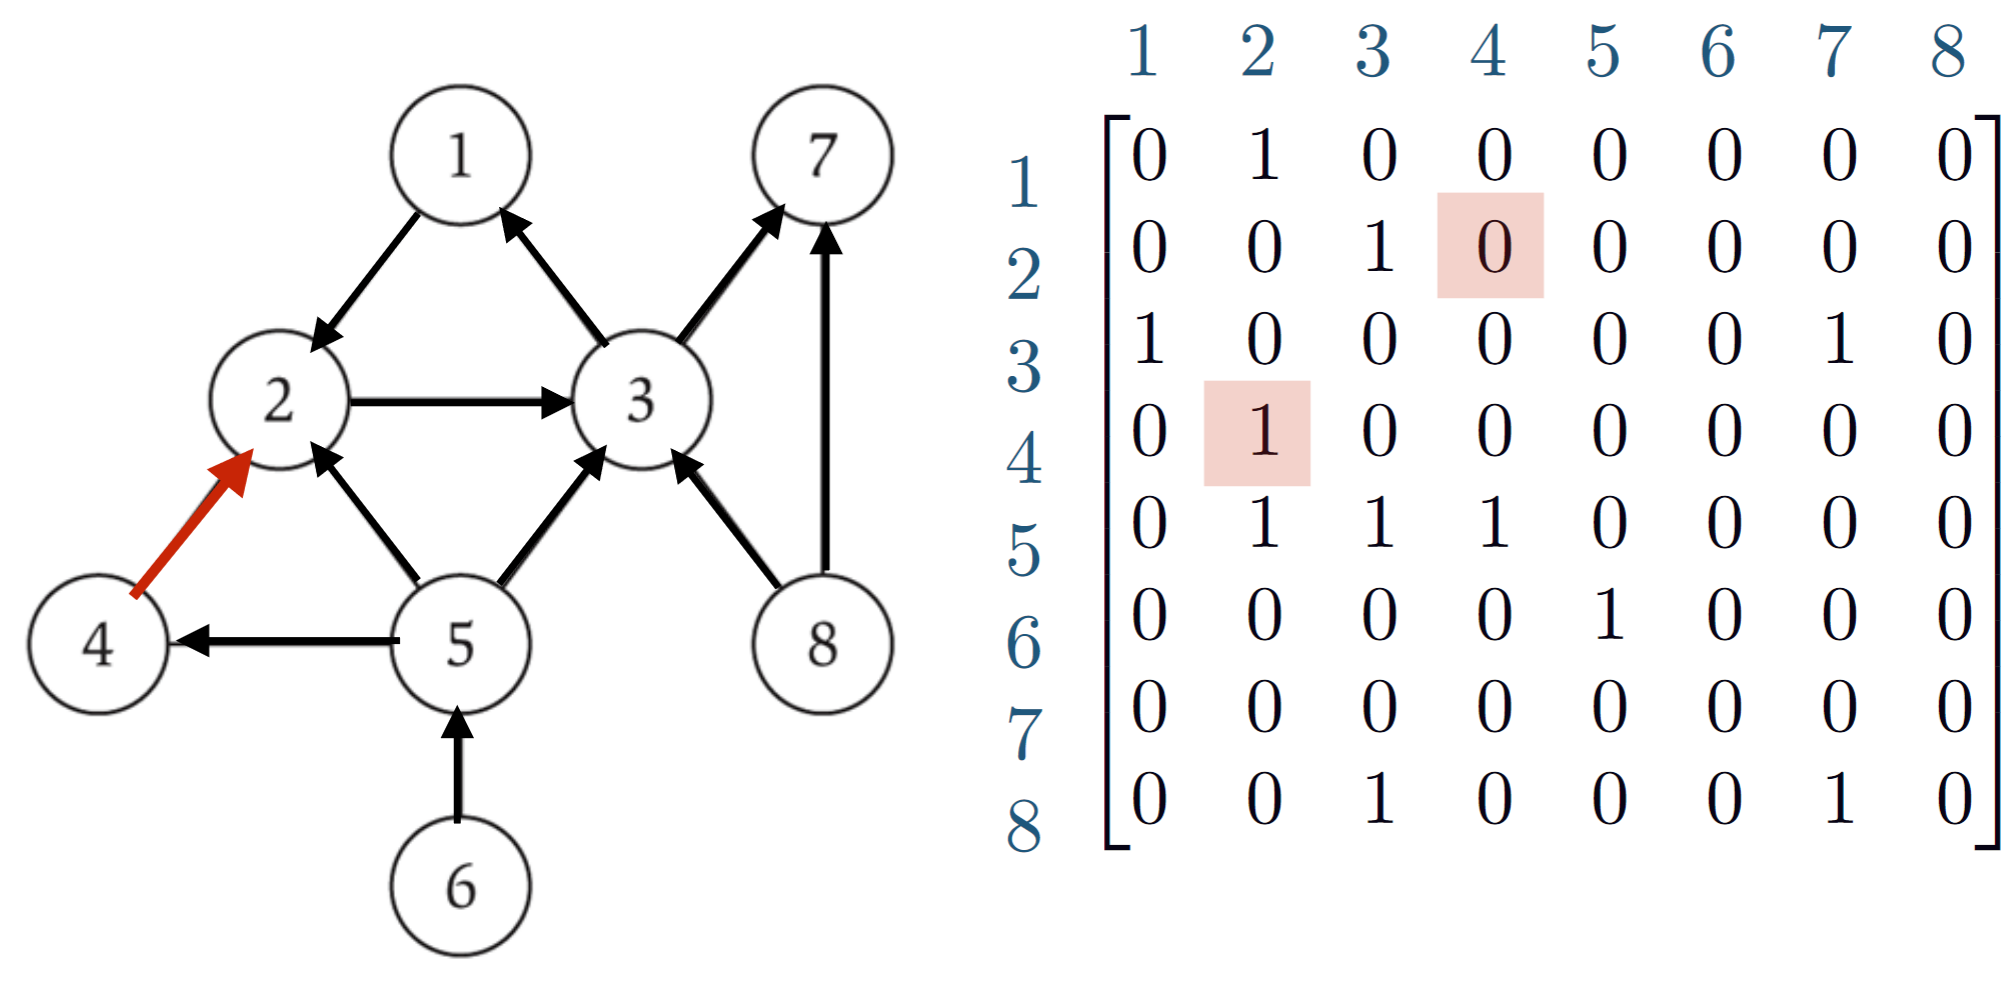
\includegraphics[height=1.5in]{./Sections/graphs/adj_matrix_dir.png}
  \end{center}
   \caption{An adjacency matrix for a directed graph with path $4\leftrightarrow2$ highlighted ($A[2][4]$ and $A[4][2]$).}\label{fig:adj_matri_dir}
\end{figure}

\newpage
\begin{Def}[Adjacency List]

  \label{def:adj_list}
    An \textbf{adjacency list} is a list of keys where each key has a list of neighbors.\\

    \noindent
    Often taking form as a dictionary or hash-table:\\
    \textbf{Space Complexity:} $\Theta (n+m)$ for $n$ nodes and $m$ total edges; \textbf{Time Complexities:}\\
    \textbf{Index key:} $\Theta (1)$; \textbf{List key neighbors:} $\Theta(\text{\# of outdegrees})$; \textbf{List all edges:} $\Theta(n+m)$;
    \textbf{Insert edge:} $\Theta(1)$. \textbf{Note:} $m\leq n^2$ (all nodes connected to all nodes), though typically $m < n$.
\end{Def}

\begin{figure}[h]
  \begin{center}
    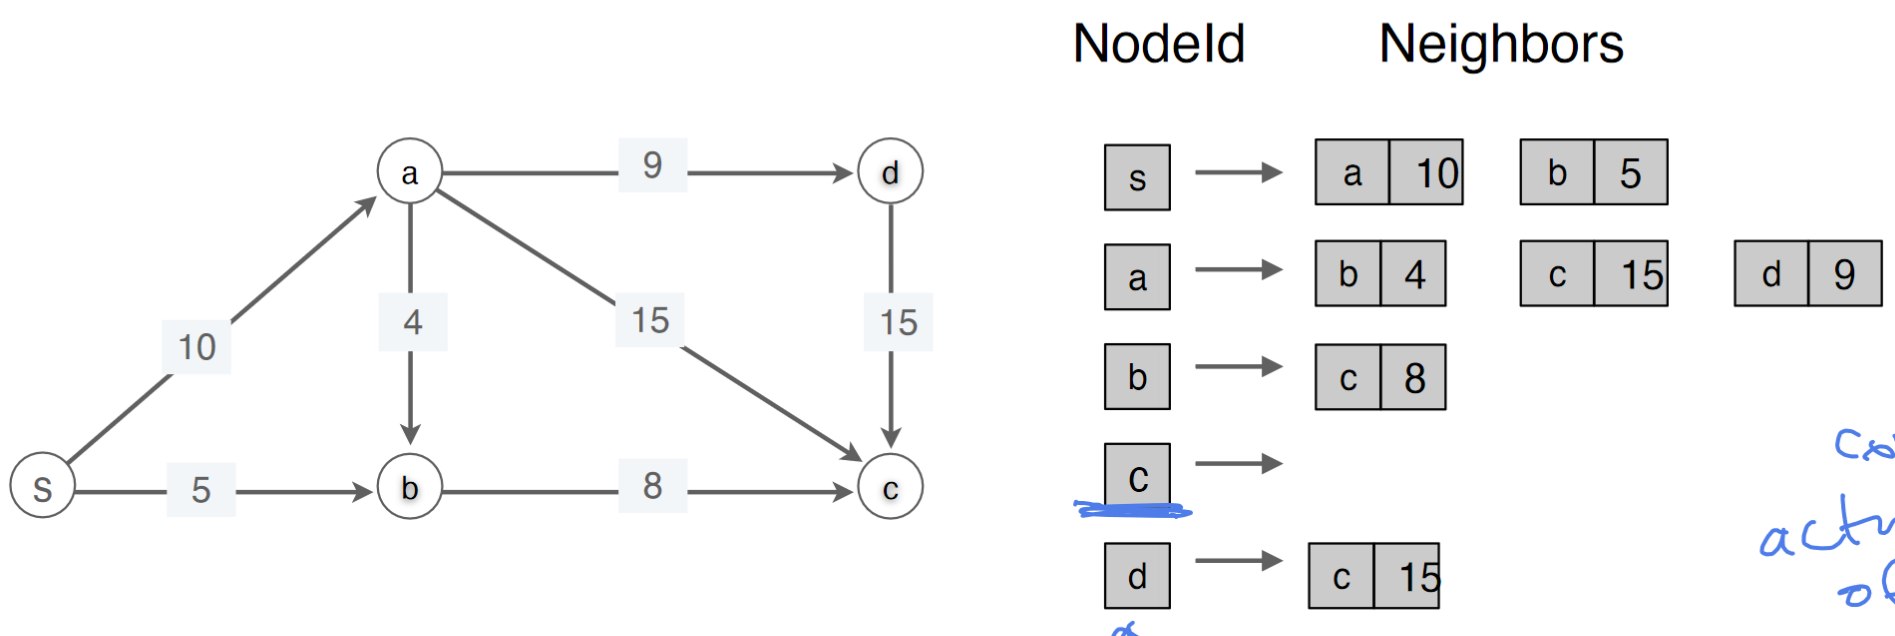
\includegraphics[height=1.5in]{./Sections/graphs/adj_list.png}
  \end{center}
   \caption{An adjacency list of a directed graph, $c$ highlighted with no outdegrees.}\label{fig:adj_list}
\end{figure}






